\documentclass[11pt,a4paper]{article}
\usepackage{stc-common}
\geometry{margin=25mm,headheight=14pt,footskip=11mm}
\linespread{1.05}
\addbibresource{bibliography.bib}
\addbibresource{source-registry.bib}

\hypersetup{
  pdftitle={Sleep-Time Compute: A Conditional Scaling Axis for Persistent AI Memory},
  pdfauthor={Samsung SAIT Neural Memory Study},
  pdfsubject={Conference manuscript on deferred learning, memory systems, and scaling hypotheses},
  pdfkeywords={sleep-time compute, continual learning, agent memory, scaling law, memory systems}
}

\title{\sffamily\bfseries\color{STCNavy}
Sleep-Time Compute:\\
지속형 AI 기억을 위한 조건부 Scaling Axis}
\author{Samsung SAIT Neural Memory Study}
\date{Source freeze: 2026-08-05}

\begin{document}
\maketitle
\begin{abstract}
Persistent AI는 release-time training과 current-query inference 사이에서 accumulated wake experience를
later-wake reusable state로 전환해야 한다. 본 논문은 이 deferred lifecycle을 sleep-time compute(STC)로
엄격히 정의하고, 73개 primary/official source의 date-frozen audit를 strongest alternatives와 비교한다.
공개 증거는 external background synthesis에는 production maturity가 있지만 broad per-user foundation-weight
sleep에는 없음을 보인다. 이에 따라 auditable external system-of-record에서 stable high-reuse subset만
reversible parametric state로 승격하는 hybrid를 조건부 base case로 제시한다. Universal scaling law는
주장하지 않고 complete-state identities, reuse/cadence break-even, capacity knee, state-migration crossover와
이를 반증할 repeated-cycle benchmark를 도출한다. 결과는 STC라는 명칭의 승리보다 multi-clock,
multi-medium memory lifecycle이 주류가 될 가능성을 지지한다.
\end{abstract}

\begin{center}
\small\sffamily
Artifact set: 70-page Full Study · separate Conference Appendix · 57-page Training Background
\end{center}

\section{문제와 operational definition}
\label{CONF-S01}

Pre/post-training은 shared capability를 배포 전에 만든다. Test-time inference와
learning\bgref{test-time-training}은 현재 query 또는 wake episode의 latency boundary 안에서 reasoning,
retrieval, fast-state update를 수행한다. 그 사이에 persistent agent가 겪은 correction, tool outcome,
procedure와 preference를 나중 wake에 재사용 가능한 상태로 바꾸는 phase가 비어 있다.

본 논문은 STC를 다음 다섯 조건의 교집합으로 정의한다: (1) input은 실제 wake lifetime에서 축적되고,
(2) 실행은 response-critical boundary 뒤로 deferred되며, (3) 결과는 다음 wake에도 남는 reusable state이고,
(4) candidate는 validation과 publication boundary를 거치며, (5) cost와 benefit은 later-wake trace에서
측정한다. Ordinary offline batching, within-query chain-of-thought, passive cache eviction, source lineage 없는
background summary, wake data와 무관한 generic retraining은 제외한다.

\begin{figure}[htbp]
\centering
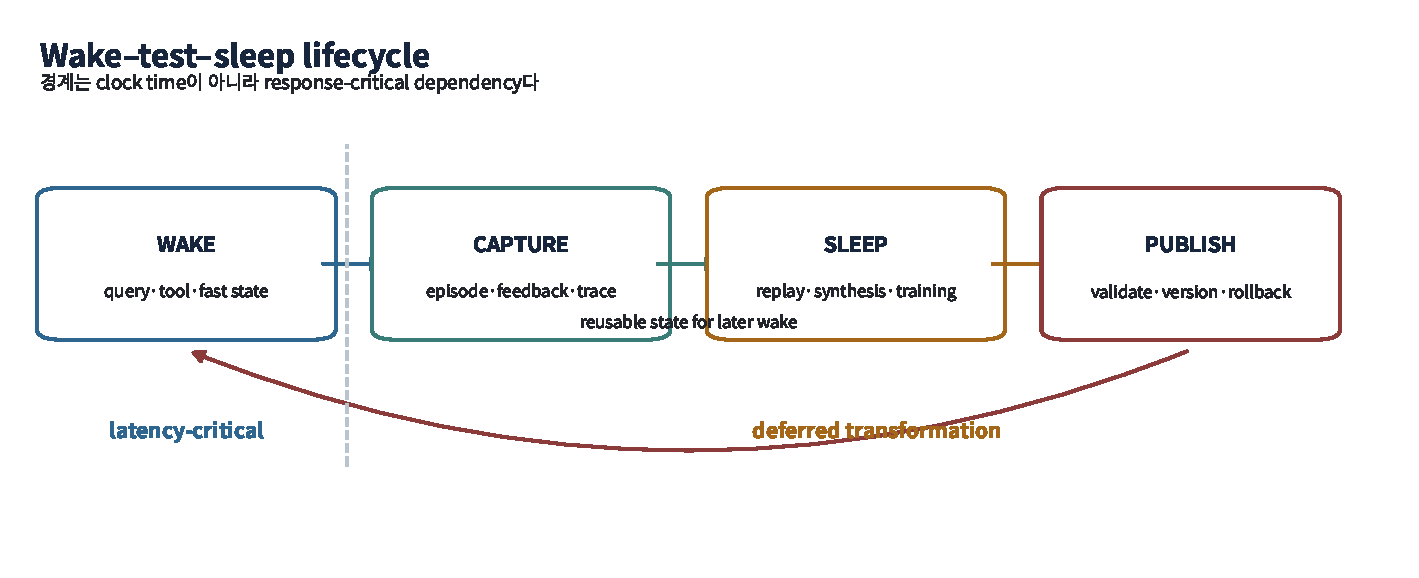
\includegraphics[width=0.92\linewidth]{figures/stc-f001.pdf}
\caption{Wake--test--sleep lifecycle과 reusable-state boundary. Sleep은 candidate를 만들 뿐 validation 전
live state를 직접 바꾸지 않는다.}
\figsource{Original synthesis; SRC-STC-0014, SRC-STC-0021, SRC-STC-0052}{Wake event가 snapshot, sleep transform, validation과 atomic publish를 거쳐 다음 wake에서 사용되는 순환 구조.}
\label{fig:conf-lifecycle}
\end{figure}

Timing과 medium은 직교한다. Sleep은 text/vector/graph external state, latent/recurrent state, LoRA
adapter\bgref{lora}, expert 또는 shared weight를 바꿀 수 있다. 반대로 같은 medium도 wake update와 sleep
update를 모두 가질 수 있다. 이 분리 없이 ``external인가 parametric인가''만 물으면 scheduling isolation,
validation과 reuse amortization의 효과를 medium 자체의 장점으로 오인한다.

\begin{table}[htbp]
\centering
\caption{본 연구의 기여와 의도적으로 남긴 non-claim}
\label{tab:conf-contributions}
\begin{tabularx}{\linewidth}{L{0.23\linewidth} Y L{0.25\linewidth}}
\toprule
기여 & 산출물 & Non-claim \\
\midrule
operational definition & causal boundary와 timing$\times$medium taxonomy & biological stage의 one-to-one 모사 \\
evidence synthesis & 73-source date-frozen claim graph & publication count 기반 trend score \\
matched decision & problem별 strongest baseline과 hybrid gate & fixed model straw-man 대비 우위 \\
scaling agenda & identity, break-even, knee, fit protocol & universal sleep-FLOP law \\
systems bridge & transactional publish와 migration accounting & 세 physical cluster가 항상 필요 \\
benchmark & repeated-cycle matched lifecycle design & 현재 production dominance 입증 \\
\bottomrule
\end{tabularx}
\end{table}

핵심 novelty는 새 optimizer 하나가 아니다. Admission, operator, destination, cadence, validation과 retirement를
하나의 lifecycle optimization으로 묶고, quality gain을 complete state와 later-wake reuse에 대해 평가하는
framing이다. 이 framing은 external-only system에도 적용되므로 parametric result가 실패해도 연구 가치가
남는다.

\section{Evidence와 strongest alternatives}
\label{CONF-S02}

2026-08-05에 동결한 73-source corpus는 biological/computational replay, continual
learning\bgref{continual-learning}, external agent memory, neural/test-time memory, product background
synthesis, capacity/security와 negative evidence를 포함한다. OpenAI Dreaming과 Mem0 Dream은 external
memory background synthesis를 공식 설명하고, Letta는 post-response asynchronous implementation을,
Zep/Graphiti는 temporal episode provenance를 공개한다.\autocite{srcstc0052,srcstc0059,srcstc0063,srcstc0065}
반면 explicit parametric sleep은 ``Language Models Need Sleep''의 research-scale evidence가 중심이다.
\autocite{srcstc0021}

Evidence maturity와 expected value를 평균하지 않았다. Product release(E4)는 lifecycle의 존재를
지지하지만 comparative optimum을 지지하지 않는다. Broad per-user weight update는 retention, delete,
rollback, security와 fleet economics를 함께 보여 주는 공개 trace가 없다. Sequential fact learning은
information이 weight에 남아도 normal behavior에서 접근 불가능해질 수 있음을 보이고, memory poisoning은
external state도 자동으로 안전하지 않음을 보인다.\autocite{srcstc0036,srcstc0042}

\begin{figure}[htbp]
\centering
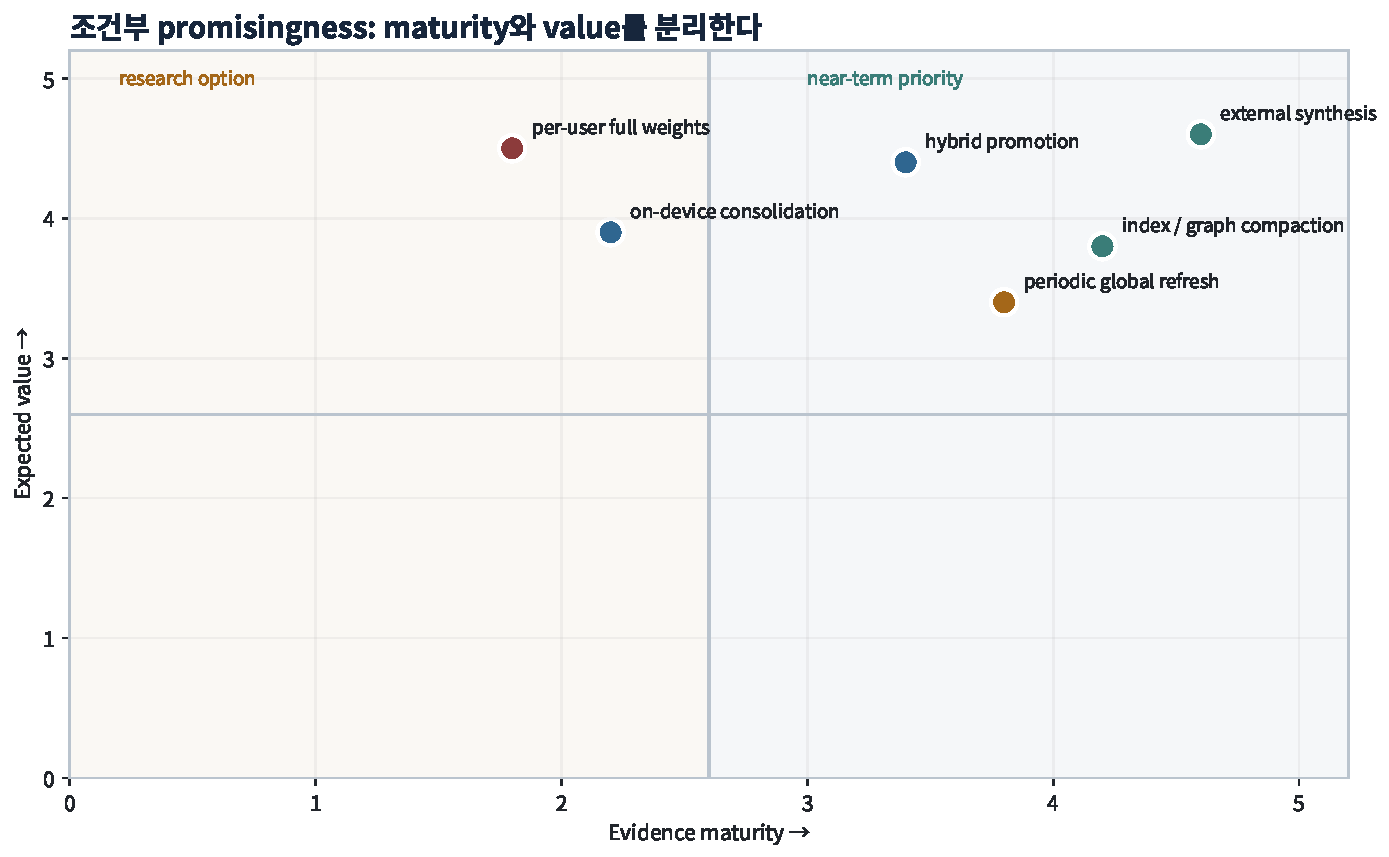
\includegraphics[width=0.89\linewidth]{figures/stc-f005.pdf}
\caption{현재의 conditional promisingness. External synthesis는 높은 maturity, selective parametric
promotion은 높은 upside와 낮은 end-to-end maturity를 갖는다.}
\figsource{Original synthesis; SRC-STC-0052, SRC-STC-0063, SRC-STC-0021}{External, learned writer, adapter promotion, broad weight update를 maturity와 expected-value 축에 놓은 산점도.}
\label{fig:conf-promisingness}
\end{figure}

\begin{table}[htbp]
\centering
\caption{Problem별 strongest non-STC baseline과 STC가 이길 조건}
\label{tab:conf-alternatives}
\begin{tabularx}{\linewidth}{L{0.20\linewidth} L{0.27\linewidth} Y}
\toprule
Problem & Strongest baseline & STC가 후보가 되는 조건 \\
\midrule
one-off long document & long context/RAG & reuse와 query predictability가 높음 \\
volatile exact fact & temporal graph/RAG & external conflict resolution; weight write는 열세 \\
repeated procedure & strategy memory/cache & held-out transfer가 compile cost를 상쇄 \\
rare factual patch & ROME/MEMIT/source edit & multi-edit integration과 validation이 필요 \\
global knowledge & periodic continued PT & local/private change가 release cadence보다 빠름 \\
continual skill & replay+PEFT/global refresh & bounded state에서 old/new/plasticity 유지 \\
serving efficiency & prefix/state cache & reusable state compatibility와 hit rate가 충분 \\
\bottomrule
\end{tabularx}
\end{table}

One-off query에서는 STC가 일반적으로 최선이 아니다. High-churn fact는 exact evidence, temporal validity와
deletion이 쉬운 external destination이 유리하다. Stable skill과 procedure는 repeated retrieval/context
cost를 parametric compile로 선불 지불할 수 있다. 따라서 가장 방어적인 구조는 external source-of-record를
유지하고, high-reuse stable subset만 versioned adapter 또는 bounded state로 승격하는 hybrid다.

\begin{figure}[htbp]
\centering
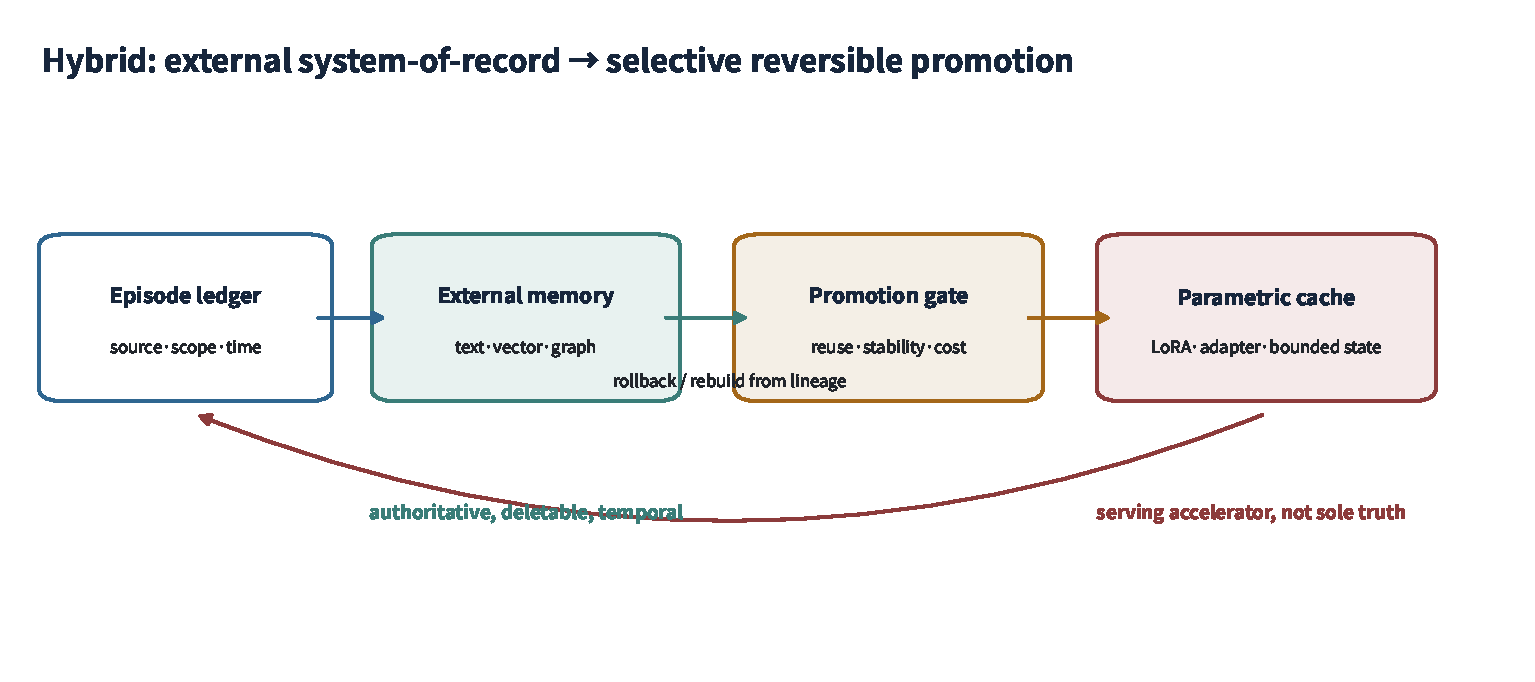
\includegraphics[width=0.94\linewidth]{figures/stc-f006.pdf}
\caption{External system-of-record와 selective reversible promotion. Parametric artifact는 authoritative
memory가 아니라 rebuild 가능한 serving cache다.}
\figsource{Original synthesis; SRC-STC-0030, SRC-STC-0066}{Canonical episode에서 external views와 promotion gate를 지나 adapter cache로 가고 lineage를 따라 rollback하는 구조.}
\label{fig:conf-hybrid}
\end{figure}

\section{Conditional mainstream verdict}
\label{CONF-S03}

현재 base case는 near-term external dominant, high-reuse domain에서 hybrid promotion으로의 진화, global
common knowledge에 대한 periodic refresh의 공존이다. STC broad adoption은 hundreds-cycle retention,
valid-reuse prediction, end-to-end delete/rollback, stable multi-resource queue, state-migration economics가
필요하다. 명칭은 dreaming, reflection, synthesis, self-evolution 또는 memory로 남을 수 있으므로 adoption은
keyword가 아니라 operational lifecycle로 추적한다.\autocite{srcstc0052,srcstc0054,srcstc0060,srcstc0063}

Mainstream confidence를 올릴 signal은 public per-user artifact lifecycle, adapter/index의 base-version churn
cost, 100--1,000 cycle retention--plasticity curve, reuse predictor calibration, derived-state delete fault
injection, background job bytes/energy/queue trace다. 반대로 validation과 state fan-out이 saved inference보다
빠르게 커지거나, high reuse에서도 external baseline과 crossover가 없으면 parametric scope를 줄여야 한다.

\begin{table}[htbp]
\centering
\caption{상호 배타적 예측이 아닌 workload-conditioned mainstream scenarios}
\label{tab:conf-scenarios}
\begin{tabularx}{\linewidth}{L{0.20\linewidth} L{0.31\linewidth} Y}
\toprule
Scenario & 성립 조건 & 가장 강한 falsifier \\
\midrule
external dominant & provenance/delete 우선, frequent base churn & stable procedure에서 persistent quality loss \\
hybrid promotion & reuse prediction, reversible adapter, lineage & dual-state/version cost가 saving을 상쇄 \\
periodic refresh & global amortization, local retention 제한 & release 사이 local procedure 변화가 큼 \\
STC niche & high reuse가 일부 domain에만 존재 & general assistant background synthesis 확산 \\
STC broad & hundreds-cycle 안정성, queue/delete/migration 해결 & validation·fan-out·privacy cost의 초과 성장 \\
\bottomrule
\end{tabularx}
\end{table}

시나리오는 같은 조직 안에서도 공존할 수 있다. Consumer factual memory는 external dominant, enterprise
procedure는 cohort adapter hybrid, universal knowledge는 periodic refresh일 수 있다. 따라서 ``STC가
mainstream인가''의 단위는 전체 모델이 아니라 workload$\times$content class$\times$destination이다.

\section{Scaling: identity, break-even, fit candidate}
\label{CONF-S04}

Universal STC scaling law는 아직 없다.\autocite{srcstc0034,srcstc0035,srcstc0050} Complete state를

\begin{equation}
B_{retained}=B_r+B_e+B_l+B_p+B_a+B_v
\end{equation}

로 기록한다. Raw evidence, external views, latent/KV, parametric state, auxiliary optimizer/router와
version/recovery를 모두 포함한다. Peak physical state는 candidate, pinned predecessor, migration,
workspace, replica, base-model residence와 execution memory를 같은 timestamp에서 더한다. Full replay는
$m_i=m$일 때 lifetime examples가 $mT(T+1)/2=\Theta(T^2)$이므로 constant admission fraction만 줄여서는
asymptotic burden이 바뀌지 않는다.

\begin{figure}[htbp]
\centering
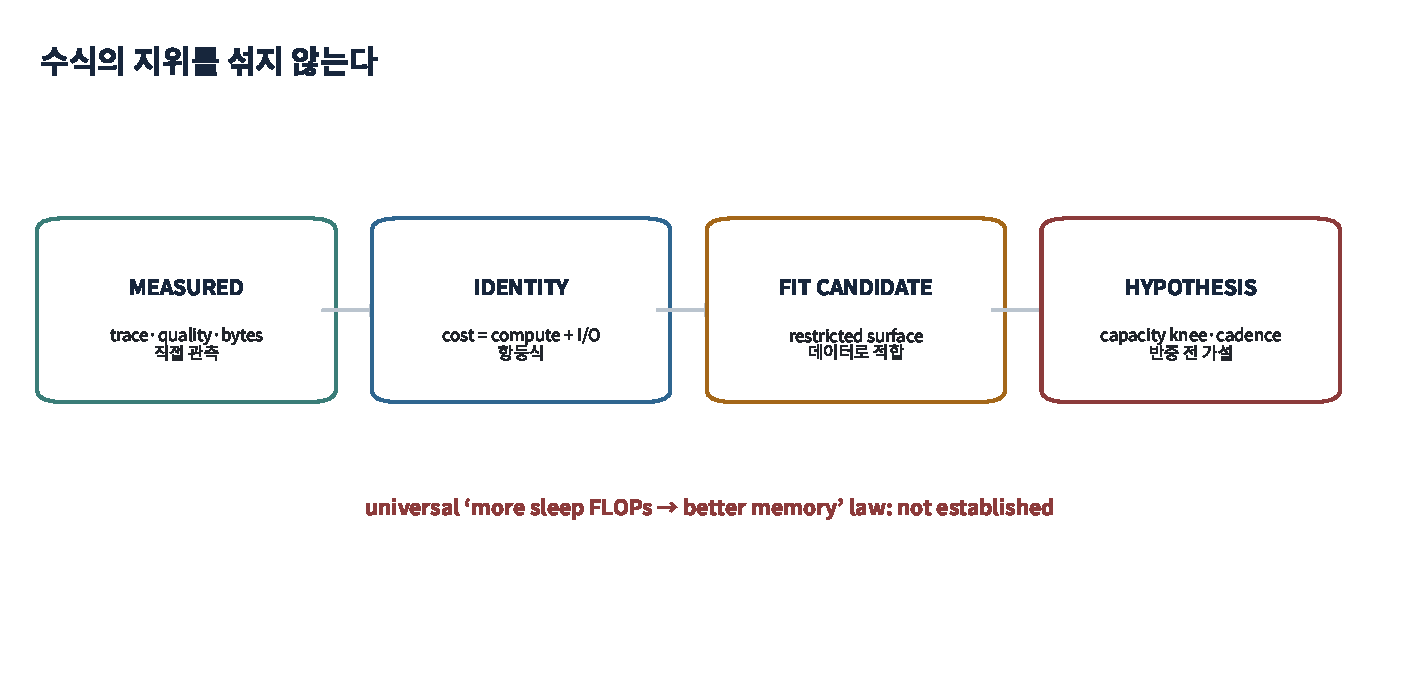
\includegraphics[width=0.89\linewidth]{figures/stc-f007.pdf}
\caption{Scaling statement의 네 등급. 보편 법칙으로 갈수록 held-out prediction과 cross-condition evidence가
추가로 필요하다.}
\figsource{Original synthesis; SRC-STC-0035, SRC-STC-0050}{Accounting identity, analytical break-even, fit candidate, untested hypothesis의 네 단계.}
\label{fig:conf-scaling-levels}
\end{figure}

Quality가 같고 use가 stationary라는 제한에서 compile reuse break-even은

\begin{equation}
n^*=\frac{C_{compile}+C_{maint}}{\Delta C_{use}}.
\end{equation}

Validity와 discount가 있으면 $R_i(H)=\int_0^H\lambda_i(t)S_i(t)e^{-\omega t}dt$를 사용한다. Promotion은
$R_i(H)\Delta U_{ij}$가 compile, serve, governance, risk의 합보다 클 때만 후보가 된다. Raw memories 또는
sleep FLOPs보다 valid reusable evidence per complete lifecycle cost가 중요한 이유다.

Cadence도 monotone하지 않다. Run cost $C_s$와 staleness $a\tau^p$의 제한된 모델은

\begin{equation}
\bar C(\tau)=\frac{C_s}{\tau}+a\tau^p,
\qquad \tau^*=\left(\frac{C_s}{ap}\right)^{1/(p+1)}
\end{equation}

를 준다. Burst, hard deadline, affinity와 capacity change에서는 queue trace로 다시 측정한다. Fixed finite
state에는 physical occupancy 전에 behavioral reachability 또는 plasticity가 무너지는 capacity knee가 있을
수 있다. 이를 global power law로 숨기지 않고 segmented/nonparametric competitor와 비교한다.

\begin{figure}[htbp]
\centering
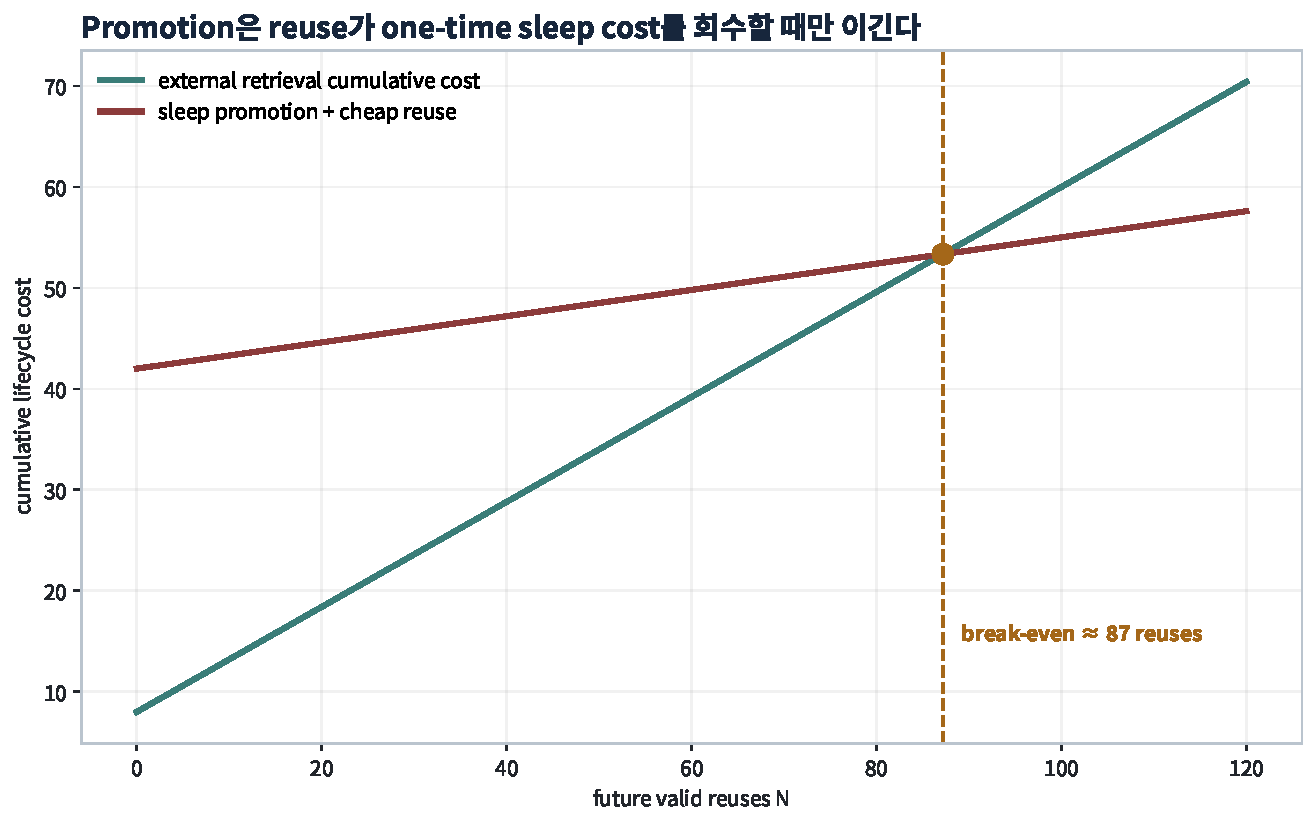
\includegraphics[width=0.88\linewidth]{figures/stc-f008.pdf}
\caption{Future valid reuse가 one-time compile cost를 상쇄하는 analytical crossover.}
\figsource{Original analytical redraw; SRC-STC-0027, SRC-STC-0052}{Compile 비용과 reuse 누적 saving의 교차점.}
\label{fig:conf-break-even}
\end{figure}

\begin{figure}[htbp]
\centering
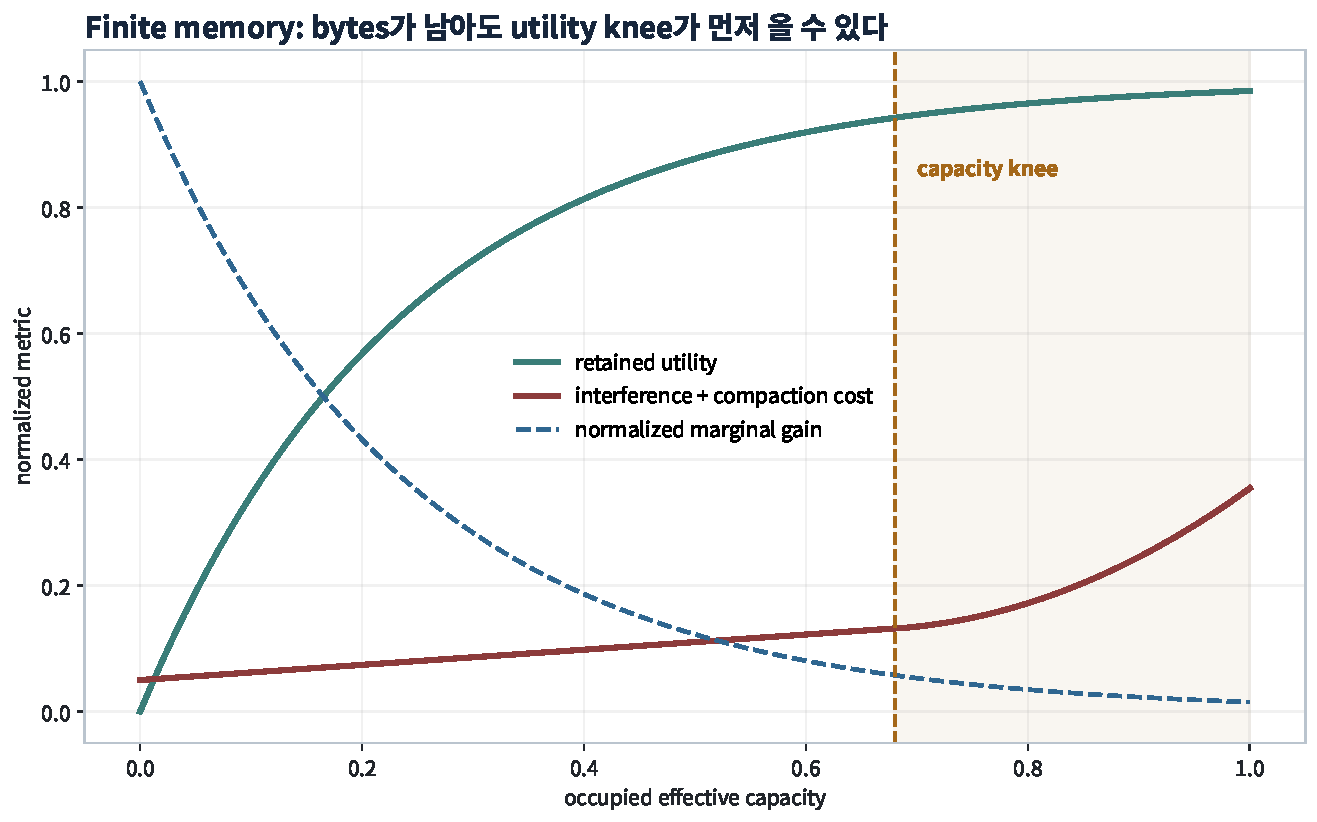
\includegraphics[width=0.90\linewidth]{figures/stc-f009.pdf}
\caption{Finite-state capacity knee hypothesis. Behavioral reachability와 plasticity는 physical occupancy보다
먼저 임계값을 넘을 수 있다. 곡선은 측정 결과가 아니라 preregistration target이다.}
\figsource{Original hypothesis redraw; SRC-STC-0034, SRC-STC-0036}{Evidence load에 따라 retention과 plasticity가 서로 다른 knee에서 감소하는 곡선.}
\label{fig:conf-capacity-knee}
\end{figure}

Cadence 식의 실험적 의미는 per-event, fixed interval, queue pressure, capacity trigger, learned policy를
같은 admitted evidence와 destination에서 비교하는 것이다. Staleness뿐 아니라 sleep job fixed cost,
batch efficiency, old-task interference, wake P99를 함께 기록해야 한다. Average utilization이 1보다 낮아도
state affinity와 validator 병목 때문에 P99 age가 발산할 수 있다.

\begin{figure}[htbp]
\centering
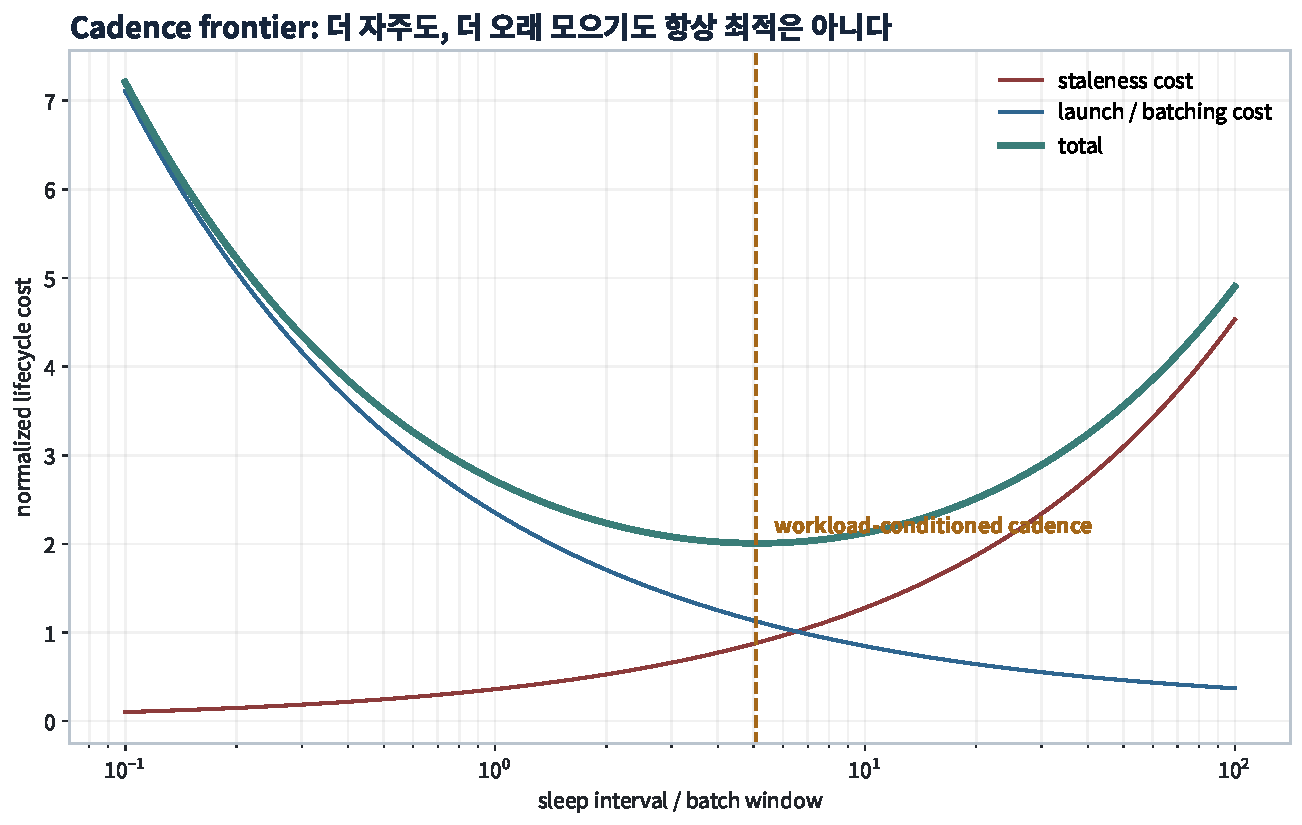
\includegraphics[width=0.90\linewidth]{figures/stc-f010.pdf}
\caption{Cadence frontier. 짧은 interval의 overhead와 긴 interval의 staleness가 내부 optimum을 만든다.}
\figsource{Original analytical redraw; SRC-STC-0020, SRC-STC-0063}{Batching cost와 staleness cost의 합이 U자 곡선을 만드는 설계 공간.}
\label{fig:conf-cadence}
\end{figure}

첫 fit candidate는

\begin{equation}
\Delta U=A\left[1-e^{-kF_s^{\alpha}E_{eff}^{\beta}R_v^{\gamma}}\right]
-\Phi_{int}-\Phi_{stale}-\Phi_{risk}
\end{equation}

처럼 evidence quality와 reuse를 분리하고 interference, staleness, risk를 뺀다. 이는 law가 아니다. 둘 이상의
model, workload, medium, hardware에서 strongest baseline과 total lifecycle cost를 맞추고 held-out condition을
예측하며 recursive depth와 repeated-cycle control을 통과해야 제한된 empirical law로 승격할 수 있다.

\section{Wake--sleep infrastructure와 device implication}
\label{CONF-S05}

Logical architecture는 wake plane, sleep candidate plane, memory/control plane으로 나뉜다. Sleep job은
immutable snapshot과 published manifest를 읽고 candidate만 만든다. Validation 뒤 complete serving head를
compare-and-swap하며, delete/authorization epoch가 중간에 바뀌면 publish가 실패한다. External raw evidence는
허용 기간 동안 source-of-record이고, summary, index, graph, latent state와 adapter는 lineage를 가진
materialized view다.

Separate sleep cluster가 항상 효율적인 것은 아니다. Link별 이동 cost를

\begin{equation}
C_{move}=\sum_{\ell}(B_{\ell}p_{\ell}+T_{\ell}v_{delay})
\end{equation}

로 두고 source뿐 아니라 base model, optimizer, candidate, validation, predecessor를 센다. Shared priority,
time-partitioned, separate, shard-local placement를 P99 wake interference, sleep job age, physical peak와 total
movement로 비교한다.

\begin{figure}[htbp]
\centering
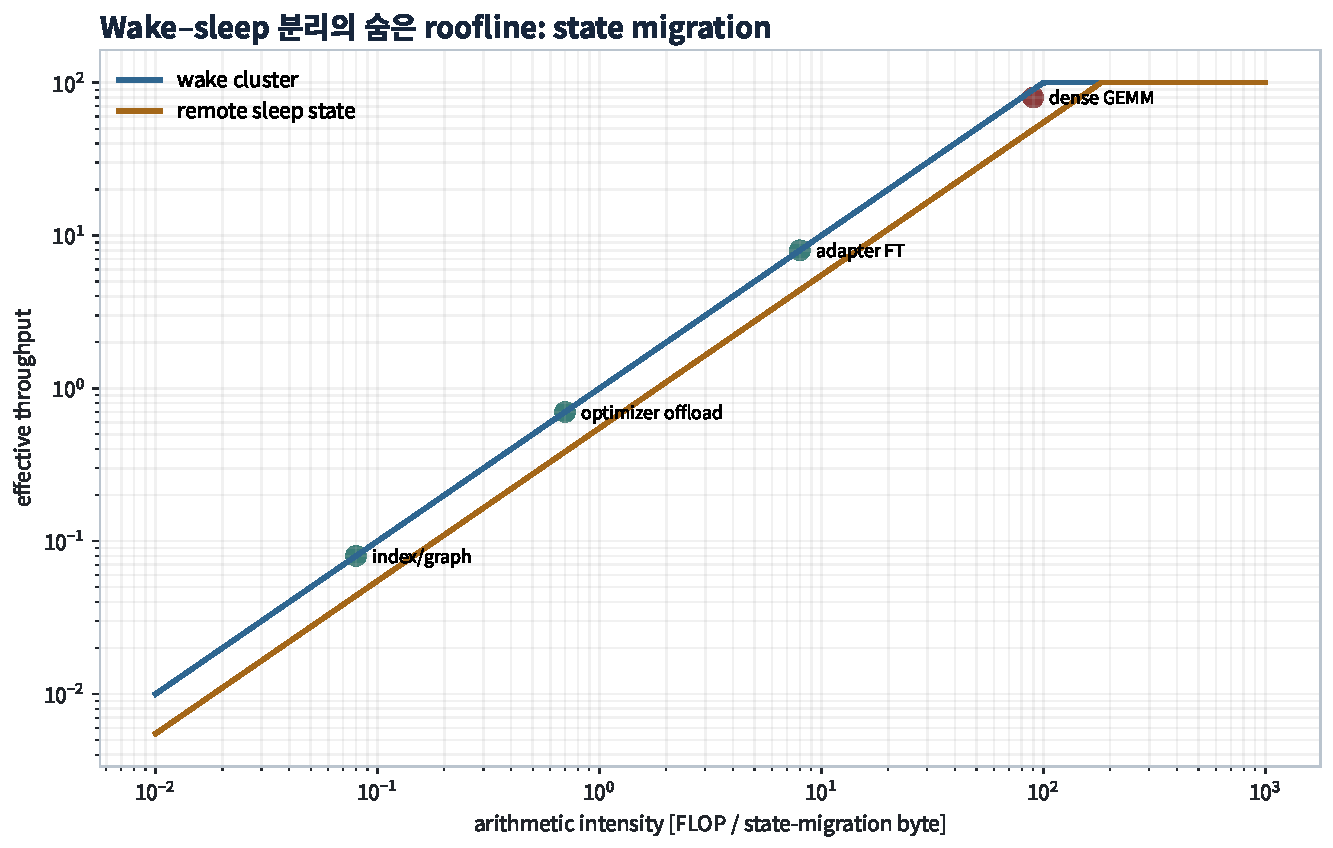
\includegraphics[width=0.91\linewidth]{figures/stc-f011.pdf}
\caption{State-migration roofline. Source-to-delta ratio, model residency와 link bandwidth가 placement
crossover를 정한다.}
\figsource{Original systems synthesis; SRC-STC-0022, SRC-STC-0059}{Shared, separate, shard-local placement의 이동량과 compute efficiency trade-off.}
\label{fig:conf-roofline}
\end{figure}

Memory-device 관점의 강건한 workload는 versioned derived state, temporal index rewrite, snapshot/COW,
heterogeneous KV/recurrent/adapter state cache, provenance lookup, secure deny/rebuild와 lifecycle telemetry다.
이 traffic은 external-dominant 미래에도 남는다. 다만 구체적 제품 hypothesis는 patent-first hold이며 이
공개 원고는 bandwidth, endurance, tail latency, bytes moved와 rollback time의 benchmark question만 제시한다.

\begin{figure}[htbp]
\centering
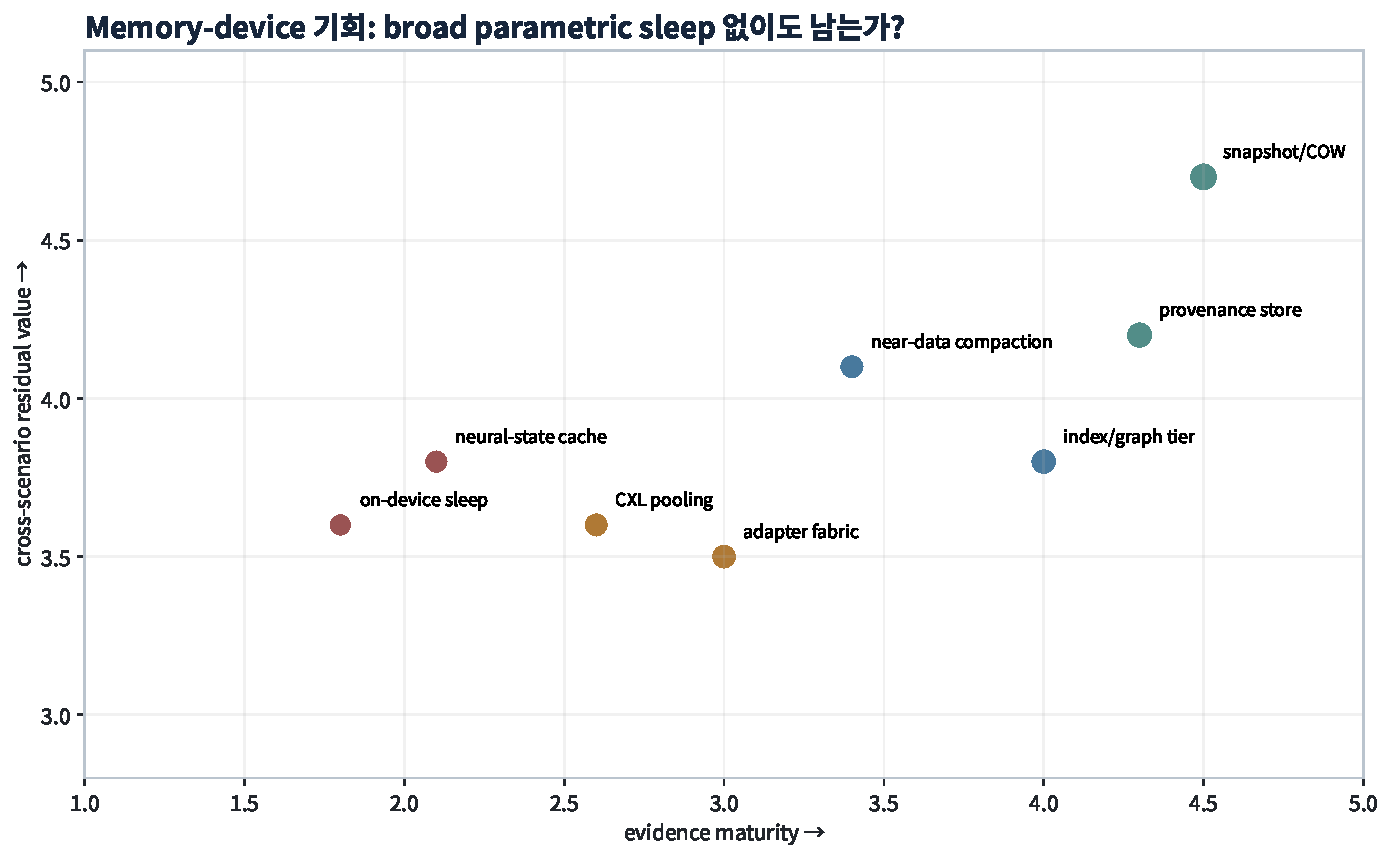
\includegraphics[width=0.90\linewidth]{figures/stc-f012.pdf}
\caption{Device research map. Evidence maturity와 STC adoption이 약해져도 남는 residual workload value를
분리한다. 좌표는 market forecast가 아니다.}
\figsource{Original research map; SRC-STC-0056, SRC-STC-0065}{Snapshot, provenance, mutable index, state cache, pooling, local compaction 후보를 두 축에 배치.}
\label{fig:conf-device-map}
\end{figure}

장치 평가는 peak GB/s 하나로 끝나지 않는다. $B_{peak,physical}$, device-level write amplification,
sequential episode scan과 random graph/index access, manifest/lineage P99, adapter page-in, secure erase,
rollback RTO를 workload phase별로 기록한다. Near-data transform은 saved link bytes에서 local execution과
validation cost를 뺀 end-to-end 결과로 판단한다.

\section{Falsifiable benchmark와 limitations}
\label{CONF-S06}

한 cycle은 wake capture, pre-sleep probe, immutable snapshot, candidate, validate/publish, post-sleep와 delayed
next-wake probe다. Default 128 cycles와 $R\in\{0,1,4,16\}$, active-capacity
$\phi\in\{1,1/4,1/16\}$을 교차한다. Raw external, compressed external, latent/KV, user LoRA, static mixture,
past-only hybrid router를 동일 event/query/resource에서 비교하며 future reuse와 correction은 oracle ledger에
격리한다.

\begin{figure}[htbp]
\centering
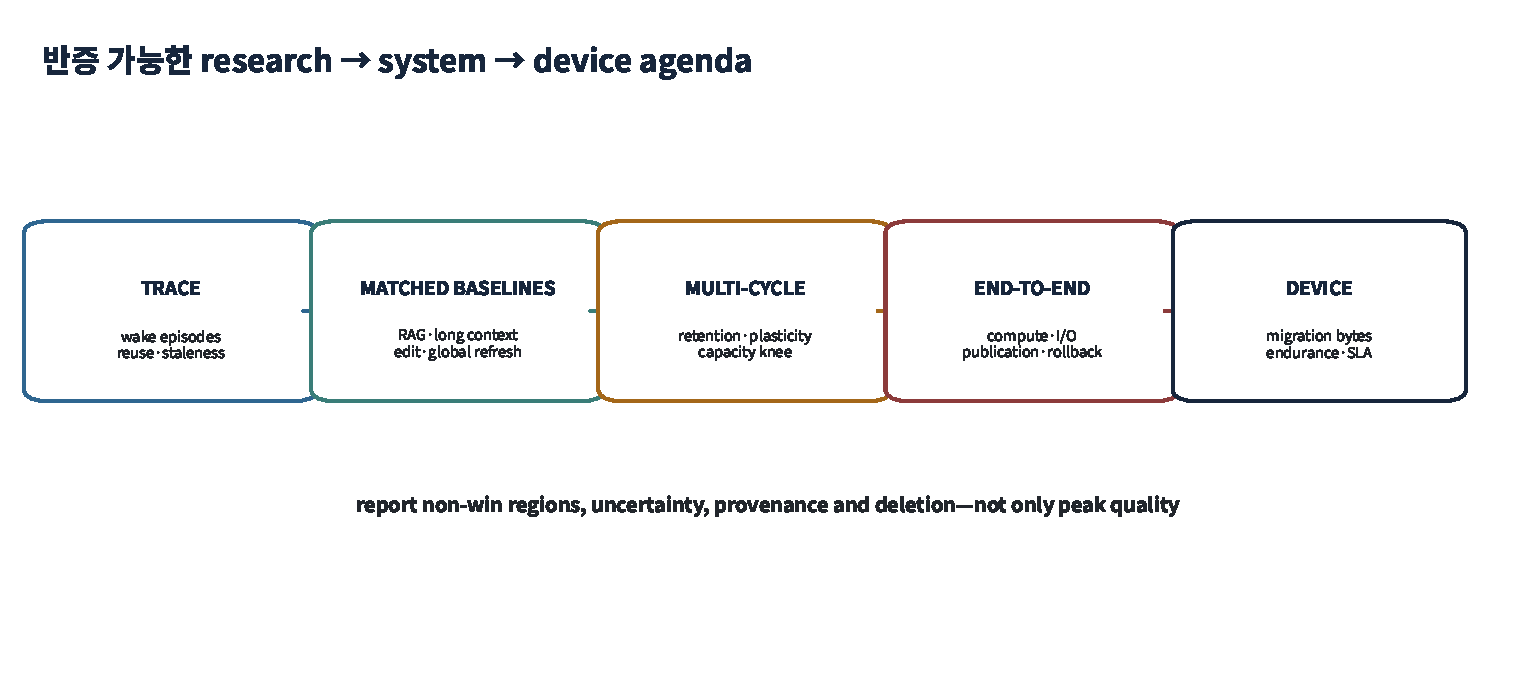
\includegraphics[width=0.94\linewidth]{figures/stc-f015.pdf}
\caption{Matched baseline에서 multi-cycle, governance, systems와 device trace로 이어지는 반증 가능한
benchmark agenda.}
\figsource{Original synthesis; SRC-STC-0036, SRC-STC-0050, SRC-STC-0056}{Trace, matched methods, repeated cycle, end-to-end control, device measurement의 순서.}
\label{fig:conf-benchmark}
\end{figure}

Metric은 lifetime utility AUC, acquisition/retention/plasticity, exact/temporal/procedural/rare-tail, false memory,
poison, access deny/physical removal/behavioral residual, TTFT/ITL, queue age, retained/peak bytes, migration,
write amplification, energy와 base compatibility를 포함한다. Timeout/OOM/deadline miss는 missing이 아니라
RESOURCE\_FAILURE로 charge한다.

본 연구는 biological stage 대응, universal monotone law, parametric dominance, product comparative
optimality를 주장하지 않는다. DANN/SSRN record는 full method와 result가 없어 load-bearing evidence에서
제외했다.\autocite{srcstc0039} Search는 date-bounded snapshot이며 5 active frontier와 5 measurement gap을
남긴다. 100--1,000 cycle, independent product evaluation, delete fault injection과 measured hardware trace가
후속 confidence를 결정해야 한다.

\begin{figure}[htbp]
\centering
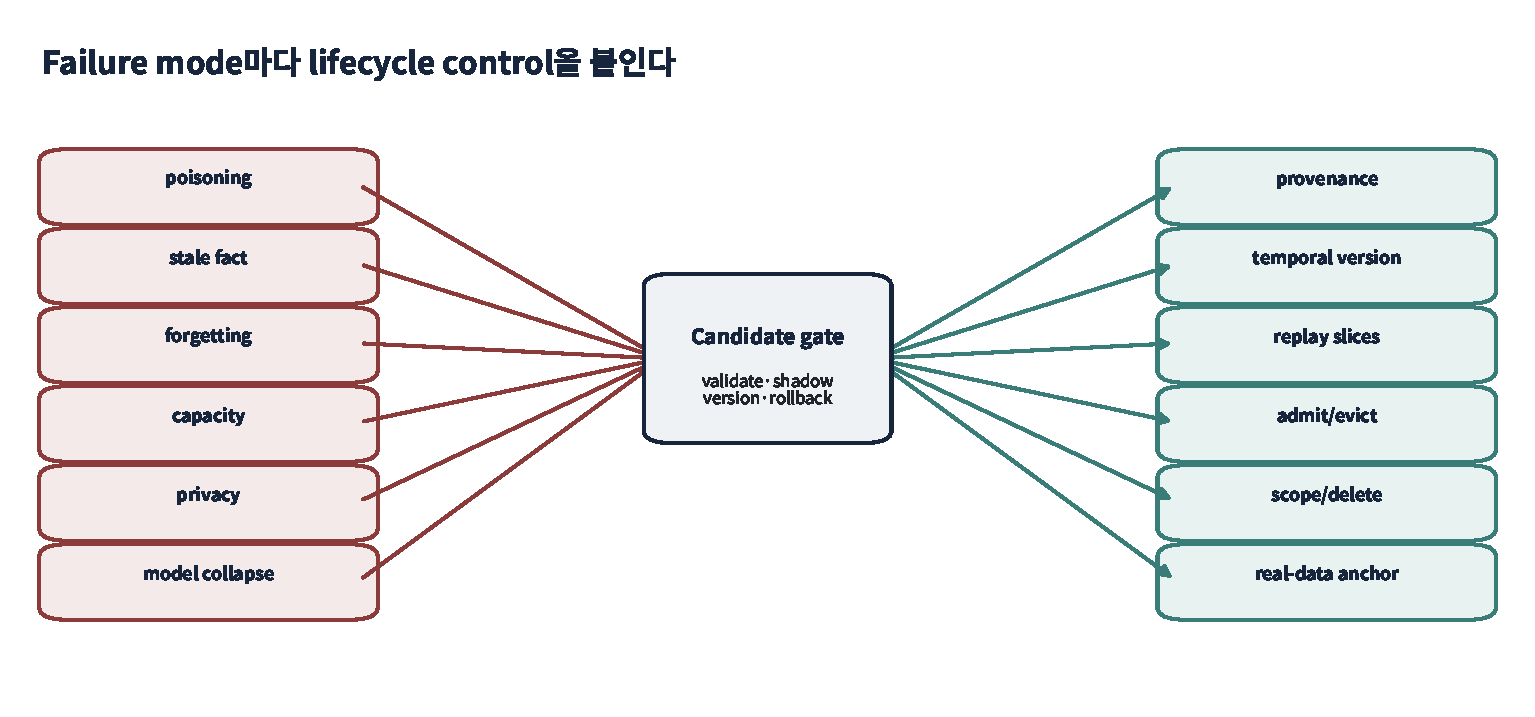
\includegraphics[width=0.91\linewidth]{figures/stc-f013.pdf}
\caption{Lifecycle failure와 control. Accuracy validation 하나만으로 poison, stale publish, rollback
resurrection과 derived-state deletion을 막지 못한다.}
\figsource{Original synthesis; SRC-STC-0042, SRC-STC-0053}{Admission부터 delete까지 failure와 provenance, quarantine, CAS, deny/rebuild control의 대응.}
\label{fig:conf-failure-controls}
\end{figure}

구체적 claim-down rule은 결과를 보기 전에 고정한다. Reuse interaction이 없으면 promotion law를,
behavioral knee가 없으면 capacity hypothesis를, shared fleet가 모든 realistic trace에서 더 낫다면 dedicated
sleep cluster를 기각한다. Archive를 보존한 active-memory 감소는 total compression이 아니며, tombstone은
physical deletion이나 unlearning이 아니다. Simulation은 특정 accelerator나 memory device의 absolute
latency/energy를 지지하지 못한다.

\section{결론}
\label{CONF-S07}

STC는 persistent AI의 실제 lifecycle 축이며 external background consolidation에서 이미 product momentum을
가진다. 그러나 continuous per-user foundation-weight update는 현재 strongest default가 아니다. 가장
유망한 다음 단계는 auditable external evidence 위의 selective reversible promotion이고, 성공 metric은
accuracy versus sleep FLOPs가 아니라 valid later-wake utility per complete lifecycle resource다. 연구의
우선순위는 더 큰 sleep model이 아니라 admission, destination, cadence, validation, retirement policy와
state movement를 함께 측정하는 것이다.

\paragraph{AI assistance disclosure.}
During the preparation of this work the authors used Codex GPT-5.6 for evidence synthesis, LaTeX drafting,
and artifact QA. All content was reviewed and edited by the authors, who take full responsibility for the
accuracy and integrity of the work.


\printbibliography[heading=bibintoc,title={참고문헌}]
\end{document}
